% Architecture diagram for the README and docs/architecture.md.
% Build: pdflatex -output-directory <tmp> architecture-diagram.tex
%        pdftocairo -svg <tmp>/architecture-diagram.pdf architecture.svg
\documentclass{article}
\usepackage[T1]{fontenc}
\usepackage{lmodern}
\usepackage{tikz}
\usetikzlibrary{arrows.meta, shapes.geometric, fit, backgrounds}
\pagestyle{empty}
\setlength{\parindent}{0pt}
\newsavebox\figbox
\pgfdeclarelayer{canvas}
\pgfsetlayers{canvas,background,main}

\begin{document}
\sbox\figbox{%
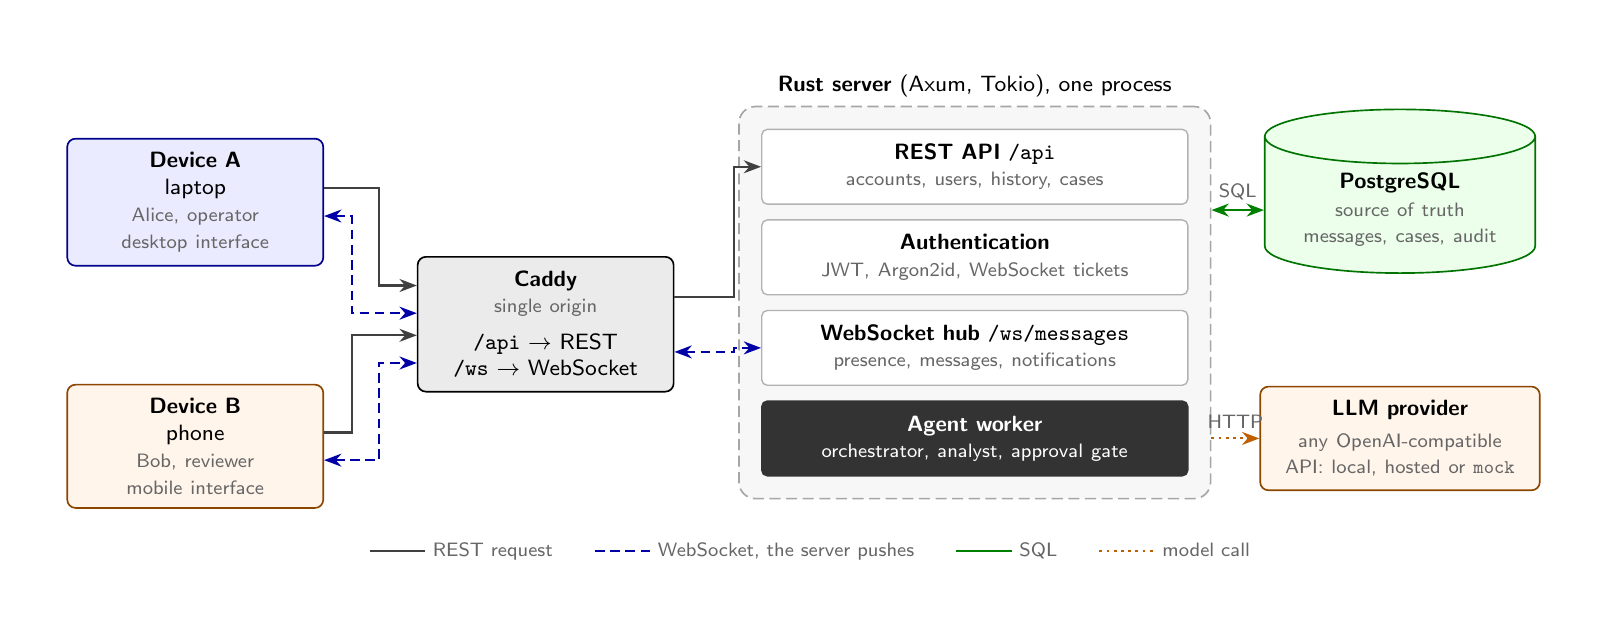
\begin{tikzpicture}[
  font=\sffamily\footnotesize,
  >={Stealth[length=2.2mm]},
  box/.style={draw=#1!55!black, fill=#1!8, rounded corners=3pt, line width=0.6pt, align=center, inner sep=5pt},
  part/.style={draw=black!30, fill=white, rounded corners=2pt, line width=0.5pt, align=center, text width=5.2cm,
    minimum height=0.95cm, inner sep=3pt},
  note/.style={font=\sffamily\scriptsize, text=black!60},
  rest/.style={->, line width=0.75pt, black!75},
  ws/.style={<->, line width=0.75pt, blue!65!black, dash pattern=on 3.5pt off 2pt},
  sql/.style={<->, line width=0.75pt, green!50!black},
  llm/.style={->, line width=0.75pt, orange!75!black, dash pattern=on 1pt off 1.6pt},
]

% Clients
\node[box=blue, text width=2.9cm] (A) at (1.3,3.3)
  {{\bfseries Device A}\\laptop\\[2pt]{\scriptsize\color{black!60} Alice, operator\\desktop interface}};
\node[box=orange, text width=2.9cm] (B) at (1.3,0.2)
  {{\bfseries Device B}\\phone\\[2pt]{\scriptsize\color{black!60} Bob, reviewer\\mobile interface}};

% Single origin
\node[box=black, text width=2.9cm] (caddy) at (5.75,1.75)
  {{\bfseries Caddy}\\{\scriptsize\color{black!60} single origin}\\[4pt]{\ttfamily /api} $\to$ REST\\{\ttfamily /ws} $\to$ WebSocket};

% Rust server
\node[part] (api) at (11.2,3.75) {{\bfseries REST API} \texttt{/api}\\{\scriptsize\color{black!60} accounts, users, history, cases}};
\node[part] (auth) at (11.2,2.6) {{\bfseries Authentication}\\{\scriptsize\color{black!60} JWT, Argon2id, WebSocket tickets}};
\node[part] (hub) at (11.2,1.45) {{\bfseries WebSocket hub} \texttt{/ws/messages}\\{\scriptsize\color{black!60} presence, messages, notifications}};
\node[part, draw=black!80, fill=black!80, text=white] (worker) at (11.2,0.3)
  {{\bfseries Agent worker}\\{\scriptsize orchestrator, analyst, approval gate}};
\begin{scope}[on background layer]
  \node[draw=black!35, fill=black!3, rounded corners=6pt, dash pattern=on 4pt off 2pt, line width=0.6pt,
        fit=(api)(worker), inner xsep=8pt, inner ysep=8pt] (server) {};
\end{scope}
\node[anchor=south, inner sep=3pt] at (server.north) {{\bfseries Rust server} (Axum, Tokio), one process};

% Storage and model
\node[cylinder, shape border rotate=90, aspect=0.2, draw=green!45!black, fill=green!8, line width=0.6pt,
      text width=3.2cm, minimum height=1.9cm, align=center] (db) at (16.6,3.2)
  {{\bfseries PostgreSQL}\\[2pt]{\scriptsize\color{black!60} source of truth\\messages, cases, audit}};
\node[box=orange, text width=3.2cm] (model) at (16.6,0.3)
  {{\bfseries LLM provider}\\[2pt]{\scriptsize\color{black!60} any OpenAI-compatible API: local, hosted or \texttt{mock}}};

% Clients to the single origin: a REST request and a WebSocket on each side
\draw[rest] ([yshift=5pt]A.east) -- ++(0.7,0) |- ([yshift=14pt]caddy.west);
\draw[ws]   ([yshift=-5pt]A.east) -- ++(0.35,0) |- ([yshift=4pt]caddy.west);
\draw[rest] ([yshift=5pt]B.east) -- ++(0.35,0) |- ([yshift=-4pt]caddy.west);
\draw[ws]   ([yshift=-5pt]B.east) -- ++(0.7,0) |- ([yshift=-14pt]caddy.west);

% Proxy to the server parts
\draw[rest] ([yshift=10pt]caddy.east) -- ++(0.75,0) |- (api.west);
\draw[ws]   ([yshift=-10pt]caddy.east) -- ++(0.75,0) |- (hub.west);

% Server to storage and model
\draw[sql] (server.east |- db.west) -- node[above, note] {SQL} (db.west);
\draw[llm] (server.east |- model.west) -- node[above, note] {HTTP} (model.west);

% Legend
\node[note, anchor=north] at (9.1,-0.9) {%
  \tikz[baseline=-0.6ex]\draw[rest,-] (0,0) -- (0.7,0); REST request\qquad
  \tikz[baseline=-0.6ex]\draw[ws,-] (0,0) -- (0.7,0); WebSocket, the server pushes\qquad
  \tikz[baseline=-0.6ex]\draw[sql,-] (0,0) -- (0.7,0); SQL\qquad
  \tikz[baseline=-0.6ex]\draw[llm,-] (0,0) -- (0.7,0); model call};

% White canvas, so the figure stays readable on a dark GitHub theme
\begin{pgfonlayer}{canvas}
  \fill[white, rounded corners=10pt] ([shift={(-14pt,-14pt)}]current bounding box.south west)
    rectangle ([shift={(14pt,14pt)}]current bounding box.north east);
\end{pgfonlayer}
\end{tikzpicture}}%
\pdfpagewidth=\wd\figbox
\pdfpageheight=\dimexpr\ht\figbox+\dp\figbox\relax
\hoffset=-1in \voffset=-1in
\oddsidemargin=0pt \topmargin=0pt \headheight=0pt \headsep=0pt \topskip=0pt
\usebox\figbox
\end{document}
